\documentclass[12pt, a4paper]{report}
\usepackage[italian]{babel}
\usepackage[T1]{fontenc}
\usepackage[sfdefault]{noto}
\usepackage{graphicx}
\usepackage{multirow}
\usepackage{enumitem}
\usepackage{hyperref}
\hypersetup{pdfborder = 0 0 0 }
\usepackage{wrapfig}
\usepackage{color}
\usepackage{tabularx}
\usepackage{makecell}
\usepackage{fancyhdr}
\linespread{1.3}
\textwidth=450pt\oddsidemargin=0pt
\begin{document}
\begin{titlepage}
\vspace{15mm}
\begin{center}
  
\includegraphics{Images/uniboLogo}
\end{center}
\begin{center}
{\normalsize{\bf Corso di Laurea Magistrale in Informatica}}\\
\vspace{5mm}
{\normalsize{\bf Anno Accademico 2018/2019}}\\
\vspace{20mm}
{\Large{\bf Software Architecture}}\\
\vspace{10mm}
{\Huge{\bf Kubernetes}}\\
\vspace{25mm}
\end{center}
\begin{center}
{\large{Matteo Marchesini\\0000856336\\matteo.marchesini12@studio.unibo.it}}
\end{center}
\end{titlepage}
\tableofcontents
\chapter{Descrizione del sistema}
\begin{center}
  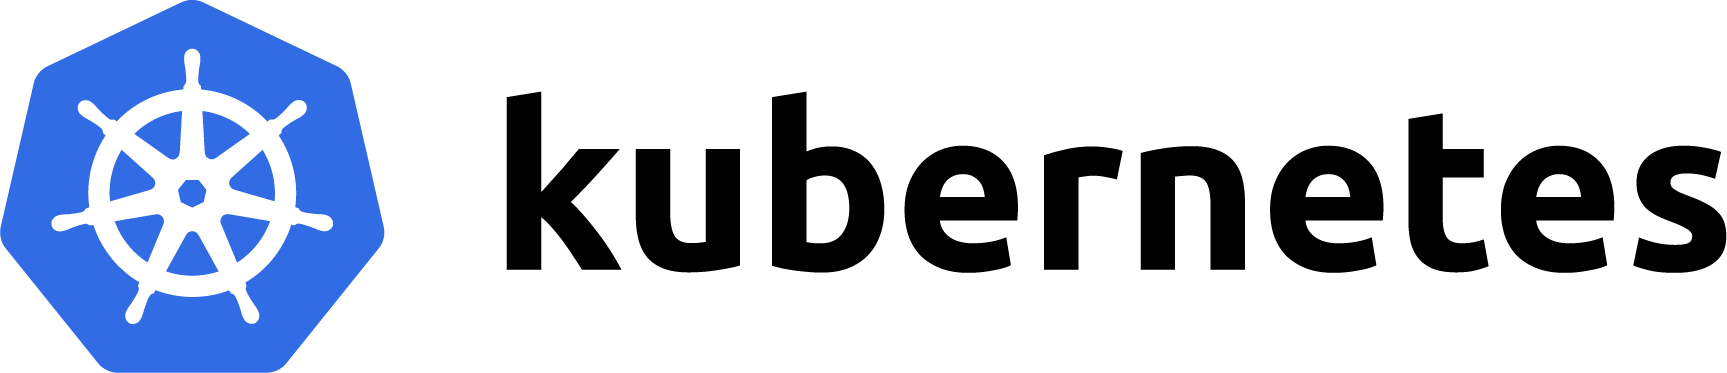
\includegraphics[scale = 0.9]{Images/kubernetesLogo}
\end{center}
Kubernetes è un sistema open source per la gestione di applicazioni containerizzate tra più host; fornisce un meccanismo per il deployment, la manutenzione e lo scaling di applicazioni. È stato inizialmente sviluppato dal team di Google, per poi passare nel 2015 sotto il controllo del \textit{Cloud Native Computing Foundation (CNCF)}, che attualmente lo supporta.\\ Al giorno d'oggi è uno dei sistemi di orchestrazione per applicazioni conteinerizzate più utilizzato in assoluto, con una vastità di utenti, partners e una comunità di development attiva. Non a caso tre dei quattro maggior providers di servizi Cloud - Microsoft, IBM e Google - offrono piattaforme di Container as a Service (CaaS) basate su Kubernetes. I servizi che Kubernetes mette a disposizione sono molteplici: fornisce un ambiente la gestione di container, microservizi e piattaforme cloud. Inoltre organizza l'infrastruttura di rete e di archiviazione per conto dell'utente.\\
In generale un sistema distribuito necessita di più componenti per il corretto funzionamento, alcune open source e altre commerciali; invece Kubernetes da solo fornisce uno scenario in cui le componenti lavorano insieme, andando così a formare un unico componente combinando la semplicità del Platform as a Service (PaaS) con la flessibilità dell'Infrastructure as a Service (IaaS).\\
L'orchestrazione di container ha avuto un profondo impatto in ogni aspetto del software development e deployment moderno; in particolare ha influenzato l'architettura del Platform as a Service, fornendo un aperto ed efficiente modello per il packaging, deployment, isolamento, scaling e rolling upgrade. Kubernetes svolgerà un ruolo cruciale nell'utilizzo di container da parte di imprese e start-up emergenti.
\\L'oggetto di questo report è di studiare tutto ciò che riguarda e circonda l'architettura di Kubernetes.
\chapter{Contesto}
\section{Scopo del sistema}
In questo capitolo verrà discusso lo scopo di Kubernetes e la sua interazione con le entità esterne, nonchè i principali casi d'uso. \\
Kubernetes, come introdotto nel Capitolo 1, è un sistema di orchestrazione di container e per questo motivo si occupa principalmente di \textbf{deployment}, \textbf{scaling} e \textbf{management} di applicazioni containerizzate. Di seguito viene definito ognuno di questi tasks:
\begin{itemize}
\item \textbf{Deployment}: gestisce la distribuzione di applicazioni assegnando ai nodi del cluster ciascuna istanza dell'applicazione. Il deployment in Kubernetes può essere eseguito in una varietà di ambienti con pattern differenti, ed esistono appunto diversi modelli, quali:
\begin{itemize}
  \item Container as a Service (CaaS);
  \item Public Cloud - Infrastructure as a Service (IaaS);
  \item Utilizzo on-premises all'interno di data center;
  \item Deployment ibrido
\end{itemize}
\item \textbf{Scaling}: permette di ridimensionare l'applicazione a seconda delle esigenze dell'utente, andando a modificare le dimensioni del cluster e il numero di repliche dei pod. Un \textbf{pod} è il più piccolo oggetto deployabile nel modello a oggetti di Kubernetes e può incapsulare un singolo container o più container che necessitano di lavorare insieme.
\item \textbf{Management}: fornisce un'interfaccia per la gestione dei cluster e delle applicazioni containerizzate. Un cluster di Kubernetes viene ospitato e gestito da un venditore commerciale, quali ad esempio Google Container Engine (GKE), Amazon EC2 Container Service e Azure Container Service di Microsoft, che offrono servizi di CaaS nel cloud pubblico. Molti utenti hanno iniziato ad usare Kubernetes attraverso Google Container Engine, essendo uno dei primi servizi di gestione di Kubernetes nel mercato.
\end{itemize}
\section{Entità esterne}
Nella figura seguente è espresso il \textit{system context diagram} di Kubernetes, che definisce le relazioni tra esso e le entità esterne.
\begin{center}
  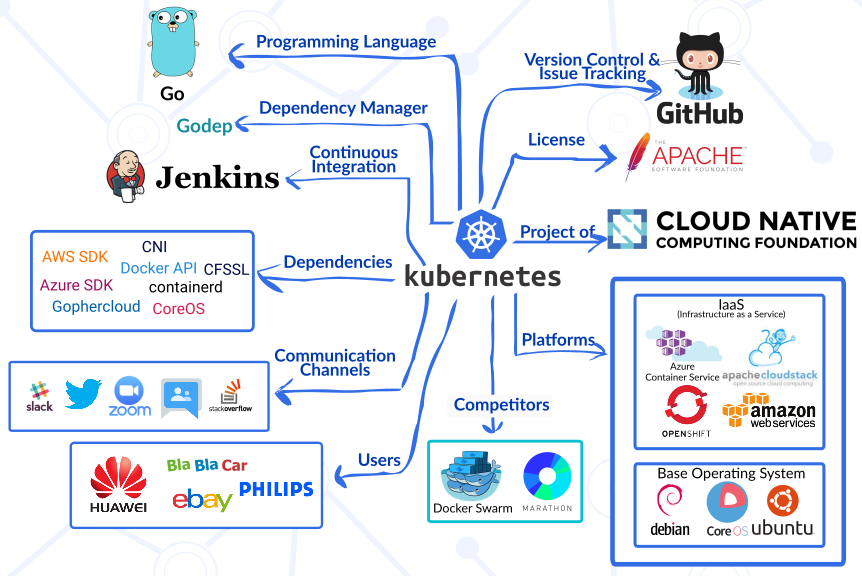
\includegraphics[scale = 0.6]{Images/ContextModelDiagram}
\end{center}
Le entità di maggior rilievo all'interno del diagramma e che verranno analizzate in seguito sono gli stakeholders, il development, le piattaforme e i concorrenti.
\subsection{Stakeholders}
Per poter comprendere al meglio il concetto di stakeholder all'interno di un progetto così grande come quello di Kubernetes, è necessario introdurre il \textbf{Cloud Native Computing Foundation} (CNCF).\\
CNCF è nato nel 2015 da un accordo tra Google e la Linux Foundation con l'annuncio di Kubernetes 1.0, considerato il progetto principale. Da li in poi molte industrie del cloud computing si sono unite a CNCF per incubare, sviluppare e mantenere un ecosistema di progetti cloud sotto una visione comune e condivisa. I membri di CNCF sono divisi per categorie, quali Platinum, Gold, Silver, End-User, accademici e no-profit. Tra i membri Platinum abbiamo Google, Docker, IBM, Cisco e Oracle.\\
Oltre all'organizzazione CNCF, Kubernetes attrae migliaia di contributori che coordinano i loro sforzi attraverso piattaforme online, quali GitHub, Slack e StackOverflow (fornitori). Gli Special Interest Groups (SIG) si occupano dello sviluppo di Kubernetes, in particolare dell'architettura, del product management e del testing, nonchè di implementazione specifiche per fornitori di servizi come AWS e Azure.
\subsubsection{Griglia Power/Interest}
Nella seguente immagine è raffigurata la griglia o matrice \textit{power/interest} che divide gli stakeholders in quattro categorie:
\begin{itemize}
  \item \textbf{Alta potenza e alto interesse}: la massima potenza suoi progetti di Kubernetes la detiene il consiglio d'amministrazione di CNCF che ne gestisce il budget, seguito poi da CNCF TOC (Technical Oversight Committee), che ha il compito di aggiungere e rimuovere progetti come Kubernetes. Inoltre anche l'architettura SIG è fondamentale in quanto decide il futuro del progetto.
  \item \textbf{Alta potenza e basso interesse}: il CNCF Marketing Committee, derivato dal consiglio di amministrazione di CNCF, cura il brand del progetto e altre attività legate al business.
  \item \textbf{Bassa potenza e alto interesse}: rispetto agli stakeholder con grande potere su Kubernetes, il CNCF end user TAB, lo staff di provider di piattaforme/servizi, Test SIG e la comunità di sviluppatori generali di Kubernetes dipendono dal continuo sviluppo del progetto, e questo comporta un alto interesse.
  \item \textbf{Bassa potenza e basso interesse}: le piattaforme di coordinamento, quali GitHub, hanno scarso potere ed interesse per il progetto, in quanto altre piattaforme potrebbero avere uno scopo simile se non fossero prese in considerazione.
\end{itemize}
\begin{center}
  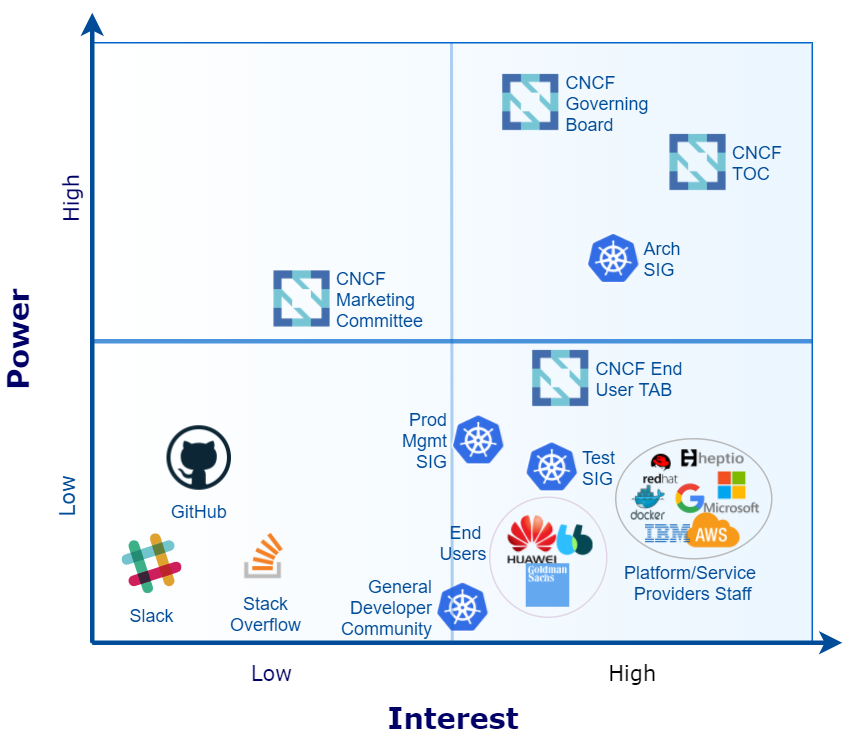
\includegraphics[scale = 0.45]{Images/power-interest}
\end{center}
\subsection{Development}
Il principale linguaggio con cui Kubernetes è sviluppato è \textbf{Go}, un linguaggio open-source progettato da tre ingegneri di Google, ma nonostante ciò possiede dipendenze da varie librerie esterne, quali Amazon Web Services SDK (AWS), Docker API, Azure SDK,  Container Network Interface (CNI), e Gophercloud. Inoltre Kubernetes si affida a Jenkins per la Continuous Integration.
\subsection{Piattaforme}
Kubernetes essendo una piattaforma cloud è compatibile con diverci providers a seconda delle necessità e dell'utilizzo. Di seguito sono riportate alcune soluzioni differenti a seconda del pattern di utilizzo.
\subsubsection{Container Management, soluzioni in locale e PaaS}
\begin{table}[ht]
  \small
  \begin{center}
  \begin{tabularx}{\textwidth}{|lr|}
    \hline
    \textbf{Prodotto} (compagnia) & \textbf{Categoria}\\
    \hline
    \textbf{AppsCode} (AppsCode)&Hosted, PaaS\\
    \multicolumn{2}{|X|}{\textit{È una piattaforma integrata per il deployment, testing e coding di app containerizzate. Permette il deployment su Google Cloud Platform e AWS.}}\\
    \hline
    \textbf{Cloud Container Engine} (Huawei)&CaaS\\
    \multicolumn{2}{|X|}{\textit{Servizio di containerizzazione scalabile ad alte prestazioni basato su Kubernetes}}\\
    \hline
    \textbf{Giant Swarm} (Giant Swarm)&Hosted, on-premises\\
    \multicolumn{2}{|X|}{\textit{Una soluzione creare, distribuire e gestire servizi containerizzati con Kubernetes come componente principale}}\\
    \hline
    \textbf{Google Container Engine} (Google)&CaaS\\
    \multicolumn{2}{|X|}{\textit{Google Container Engine è un sistema di gestione e orchestrazione dei cluster che consente agli utenti di eseguire container sulla piattaforma Cloud di Google}}\\
    \hline
    \textbf{OpenShift Container Platform} (RedHat)&PaaS, on-premises\\
    \multicolumn{2}{|X|}{\textit{Una piattaforma di applicazioni per container che può estendersi su più infrastrutture. È costruito usando la tecnologia Docker e Kubernetes.}}\\
    \hline
  \end{tabularx}
  \end{center}
\end{table}

\begin{table}[ht]
\small
\centering
\begin{tabularx}{\textwidth}{|lr|}
\hline
\textbf{OpenShift Online} (RedHat)&Hosted\\
\multicolumn{2}{|X|}{\textit{Versione hosted di OpenShift. Il funzionamento è il medesimo a quello di OpenShift Container Platform}}\\
\hline
\textbf{Platform9 Managed Kubernetes for Docker} (Platform9)&Hosted, on-premises\\
\multicolumn{2}{|X|}{\textit{I clienti possono utilizzare il singolo pannello di Platform 9 per orchestrare e gestire i container insieme alle macchine virtuali. In pratica, è possibile orchestrare le VM utilizzando OpenStack e/o Kubernetes}}\\
\hline
\end{tabularx}
\end{table}

\subsubsection{Tools per deployment e controllo di clusters Kubernetes}
\begin{table}[ht]
\small
\centering
\begin{tabularx}{\textwidth}{|lr|}
\hline
\textbf{Prodotto} (compagnia) & \textbf{Categoria}\\
\hline
\textbf{AppFormix} (AppFormix)&Monitoring\\
\multicolumn{2}{|X|}{\textit{Fornisce metriche e analisi per i container. Gli utenti possono gestire avvisi, o regole di orchestrazione per singoli pods o container. La dashboard può essere ulteriormente personalizzata e mappata nei propri progetti}}\\
\hline
\textbf{Bootkube} (CoreOS)&Deploy\\
\multicolumn{2}{|X|}{\textit{Uno strumento di supporto per l'avvio di cluster Kubernetes autogestiti.}}\\
\hline
\textbf{ElasticBox ElasticKube} (CenturyLink)&Deploy\\
\multicolumn{2}{|X|}{\textit{Un servizio per pipeline di CI/CD, per la configurazione di tools di management e per il deployment di applicazioni cloud. Include ElasticKube, una piattaforma open source per Kubernetes che promuove il self-service per le applicazioni containerizzate.}}\\
\hline
\textbf{Kubernetes Dashboard} (Cloud Native Computing Foundation)&Monitor\\
\multicolumn{2}{|X|}{\textit{Fornisce un'interfaccia utente basata sul Web per cluster Kubernetes. Consente agli utenti di gestire le applicazioni in esecuzione nel cluster nonché di gestire il cluster stesso.}}\\
\hline
\textbf{Minikube} (Cloud Native Computing Foundation)&Deploy\\
\multicolumn{2}{|X|}{\textit{Minikube è un tool che permette di eseguie in locale Kubernetes, semplicemente eseguendolo all'interno di una VM del proprio pc. }}\\
\hline
\end{tabularx}
\end{table}
\newpage
\subsubsection{Tool per integration}
\begin{table}[ht]
\small
\centering
\begin{tabularx}{\textwidth}{|l|}
\hline
\textbf{Prodotto} (compagnia) \\
\hline
\textbf{Apprenda} (Apprenda)\\
\multicolumn{1}{|X|}{\textit{Fornisce PaaS private per le aziende che supportano l'hosting di container}}\\
\hline
\textbf{Crunchy PostgreSQLContainer Suite} (Crunchy Data)\\
\multicolumn{1}{|X|}{\textit{Un set di container Docker e servizi Kubernetes "preconfezionato"; il Crunchy Container Suite permette ai team di eseguire e gestire PostgreSQL su ambienti basati su Kubernetes}}\\
\hline
\textbf{fabric8} (Red Hat)\\
\multicolumn{1}{|X|}{\textit{Una piattaforma open-source per il DevOps e integrazione costruita con un set di microservizi eseguiti su Kubernetes e OpenShift V3. La sua continuos delivery è basata su Jenkins, Nexus e SonarQube}}\\
\hline
\textbf{Kubeflix} (Red Hat)\\
\multicolumn{1}{|X|}{\textit{Integrazione di Kubernetes con i componenti open source di Netflix, quali Hystrix, Turbine e Ribbon}}\\
\hline
\textbf{NetScaler CPX} (Citrix)\\
\multicolumn{1}{|X|}{\textit{Sistema di bialnciamento della containerizzazione in Docker che può essere supportata on-premises o in ambienti multi-cloud. NetScaler CPX si integra con Kubernetes al fine di bilanciare applicazione containerizzate all'interno di cluster. Nell'ambiente di Kubernetes, NetScaler CPX rimpiazza kube-proxy nei minion e bilancia il carico nei pod. }}\\
\hline
\end{tabularx}
\end{table}
\subsection{Concorrenti}
Tra i tool concorrenti a Kubernetes che offrono un servizio di orchestrazione di container abbiamo \textbf{Docker Swarm} e \textbf{Marathon}. Marathon è una piattaforma di orchestrazione di applicazioni e servizi per Apache Mesos.\\
Docker Swarm invece, che è integrato in Docker come \textit{Swarm Mode}, è un orchestratore per i container Docker. Confrontando Docker Swarm con Kubernetes, emerge che quest'ultimo è un tool molto più efficiente, in quanto offre una maggiore scalabilità e automazione. Inoltre Kubernetes possiede delle proprie librerie per il monitoraggio e i logging; ciò viene a mancare in Docker Swarm, che deve ricorrere ad applicazioni di terze parti per sopperire a queste features.
Kubernetes supera i vincoli imposti da Docker e Docker API per il deployment, e per questo è maggiormente utilizzato. In Kubernetes se un nodo fallisce, esso viene rimpiazzato così velocemente da non accorgersi, a meno che non si esegua una dettagliata risoluzione dei problemi.
\chapter{Drivers architetturali}
Kubernetes, come si può capire dal capitolo precedente, è progettato secondo i principi di scalabilità, disponibilità e sicurezza, nonchè fornisce una distribuzione del carico di lavoro tra le risorse disponibili. Questo capitolo metterà in evidenza alcuni dei requisiti non funzionali di Kubernetes.
\section{Scalabilità}
Le applicazioni sono eseguite in Kubernetes come microservizi. Tali microservizi sono composti da più container raggruppati in \textbf{pods}. Ciascun container è progettato per eseguire solamente un unico task.\\
I pods possono essere composti da container con o senza stato (stateless/stateful). I pods senza stato possono essere scalati facilmente quando necessario anche attraverso l'auto-scaling dinamico.\\
Dalla versione 1.4 Kubernetes supporta l'auto-scaling orizzontale dei pod, che scala autmaticamente il numero di pod in repliche controllate basate sull'utilizzo della CPU. La versione di Kubernetes ospitata da Google Cloud supporta l'auto-scaling di cluster. Quando un nuovo pod viene scalato tra tutti i nodi disponibili, Kubernetes coordina l'infrastruttura sottostante per far si che ulteriori nodi vengano aggiunti al cluster. \\
\begin{figure}
  \begin{center}
  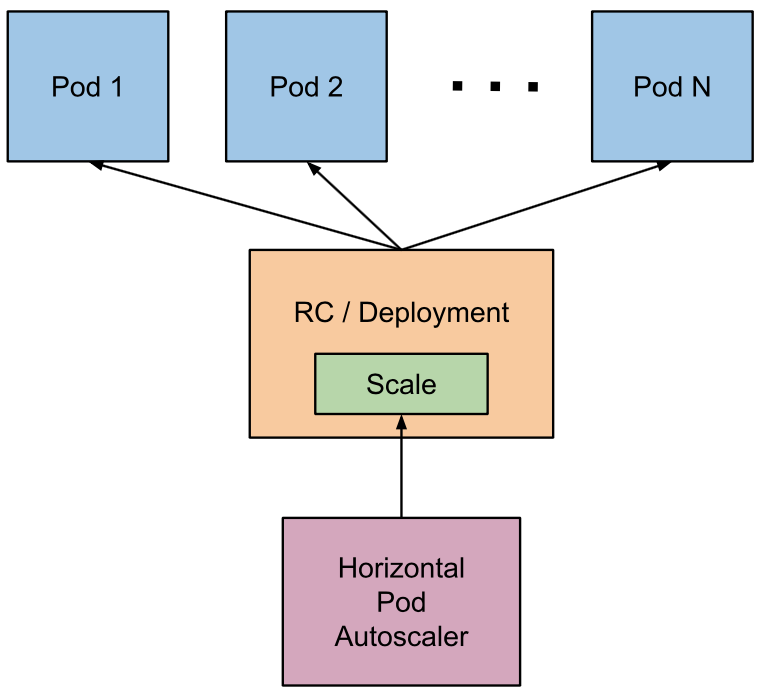
\includegraphics[scale = 0.7]{Images/horizontal-pod-autoscaler}
  \caption{Autoscaling orizzontale di un pod}
  \end{center}
\end{figure}
L'auto-scaling orizzontale è implementato come un loop di controllo, in cui periodicamente (con un valore predefinito di 30 secondi) il controller manager interroga l'utilizzo delle risorse rispetto alle metriche specificate in ciascuna definizione di \textit{HorizontalPodAutoscaler}.
Nello specifico, il controller manager ottiene le metriche (ad esempio l'utilizzo di CPU) attraverso l'API apposita per le metriche; quindi se è settato un valore target di utilizzo, il controller calcola il valore di utilizzo come percentuale delle richieste alle risorse equivalenti contenute nei container di ciascun pod. Se invece è impostato un valore grezzo, il controller utilizza direttamente tale valore. Il controller quindi assume o la media di utilizzo o il valore grezzo, per produrre poi un rapporto usato per scalare il numero di repliche desiderate. Da sottolineare il fatto che se alcuni container all'interno dei pods non hanno il set di richieste di risorse rilevanti, l'utilizzo di CPU per quel dato pod non verrà definito e l'autoscaler non intraprenderà alcuna azione per tale metrica.\\
Kubernetes supporta inolte lo scaling di applicazioni stateless come i cluster Cassandra e i set di repliche MongoDB, ovvero più in generale di workloads persistenti, quali i database NoSQL e i database relazionali (RDBMS).
\section{Disponibilità}
In kubernetes i carichi di lavoro richiedono la disponibilità sia a livello di infrastruttra che applicazione. Ad esempio, nei cluster a larga scala, tutto è soggetto ai guasti, il che rende necessaria un'elevata disponibilità per la produzione dei workloads.
Mentre la maggior parte dei motori di orchestrazione di container offrono la disponibilità di applicazioni, Kubernetes è progettato per affrontare la disponibilità sia di applicazioni che di infrastrutture.\\
Per quanto riguarda il fronte applicazione, Kubernetes assicura un alta disponibilità per mezzo di \textit{ReplicaSet}, \textit{Replication Controller} e \textit{StatefulSets}. Un ReplicaSet garantisce che un numero specificato di repliche di pod siano in esecuzione in qualsiasi momento, e lo stesso vale per i Replication Controller, con l'unica differenza che quest'ultimo supporta solo il selettore di uguaglianza, mentre ReplicaSet supporta il selettore basato sul set.\\
Quindi l'utilizzatore di Kubernetes può dichiarare il numero minimo di pods che devono essere eseguiti in un dato istante di tempo. Se un container o un pod si arresta in modo anomalo a causa di un errore, la policy dichiarativa può riportare il deployment alla configurazione desiderata.\\
Analizzando la disponibilità rispetto all'infrastruttura, Kubernetes supporta un'ampia gamma di back-end di archiviazione, quali file systems distribuiti, come il file systems di rete (\textbf{NFS}) e \textbf{GlusterFS}, gli storage persistente a livello di blocco, come \textbf{Amazon Elastic Block Store} (EBS) e Google Compute Engine, e infine container di storage come \textbf{Flocker}, un open-source Container Data Volume Manager per le applicazioni in Docker. L'aggiunta di un livello di archiviazione affidabile e disponibile a Kubernetes garantisce un'elevata disponibilità di workloads statici. Ogni componente del cluster di Kubernetes - etcd, API server, nodi - può essere configurato per garantire un alta disponibilità. Le applicazioni hanno quindi il vantaggio di usufruire di un bilanciamento del carico di lavoro e di checks di controllo per garantire disponibilità.
\section{Sicurezza}
La sicurezza in Kubernetes è configurata su più livelli. Gli endpoints dell'API sono protetti tramite Transport Layes Security (\textbf{TLS}), che garantisce l'autenticazione dell'utente utilizzando il meccanismo di autenticazione più sicuro disponibile. I cluster di Kubernetes hanno due categorie di utenti:
\begin{itemize}
  \item Service account, gestiti direttamente da Kubernetes;
  \item Utenti normali, che si suppone essere gestiti da un servizio indipendente.
\end{itemize}
I service account gestiti da Kubernetes sono creati in automatico dall'API server. Ciascuna operazione che gestisce un processo in esecuzione all'interno di un cluster deve essere avviata da un utente autenticato; questo meccanismo garantisce la sicurezza del cluster.\\
Le applicazioni eseguite all'interno di un cluster Kubernetes possono beneficiare del concetto di \textit{segreti} per un accesso sicuro ai dati. Un \textbf{segreto} è un oggetto Kubernetes che contiene una piccola quantità di dati sensibili, come password, token o chiave, che riduce il rischio di esposizione accidentale dei dati. Gli username e le password sono codificati in base64 prima di essere memorizzati all'interno del cluster Kubernetes. I pod possono accedere al segreto in fase di runtime tramite i volumi montati o le variabili d'ambiente.\\
Per permettere o limitare il traffico di rete ai pods, le politiche di rete possono essere applicate al deployment. Una policy di rete è una specifica di come i gruppi di pod possono comunicare tra loro e con altri endpoint di rete. Ciò può risultare utile in un deployment a più livelli per oscurare i pods in modo da non essere esposti ad altre applicazioni.
\begin{figure}
  \begin{center}
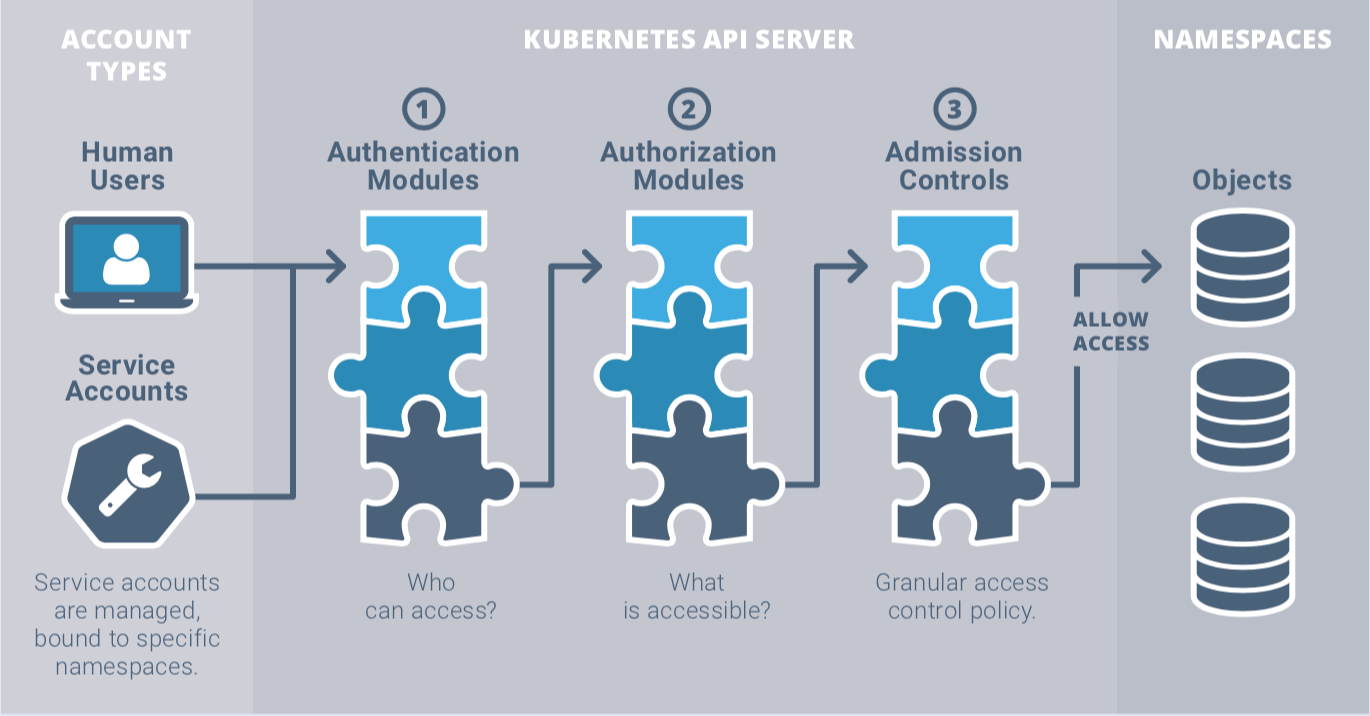
\includegraphics[scale = 0.5]{Images/Kubernetes-auth}\\
  \caption{Utilizzo dei moduli di autenticazione, autorizzazione e Admission Control per controllare l'accesso API in Kubernetes.}
  \end{center}
\end{figure}
\newpage
\section{Portabilità}
Kubernetes è progettato per offrire una libertà di scelta rispetto alla scelta del sistema operativo da utilizzare, all'esecuzione dei container, all'architettura del processore, alle piattaforme cloud e al PaaS.\\
Infatti un cluster Kubernetes può essere configurato nelle principali distribuzioni Linux, quali CentOS, CoreOS, Debian, Fedora, Red Hat Linux e Ubuntu. Può essere eseguito in locale oppure in piattaforme cloud, come AWS, Azure e Google Cloud; su ambienti virtualizzati basati su KVM e vSphere. Gli utenti possono lanciare container in Docker o rkt runtimes, e nuovi container possono essere lanciati anche a tempo di esecuzione. \\
Inoltre attraverso la \textit{federation} è anche possibile combinare cluster eseguiti tra più cloud provider differenti e in locale. Ciò porta le funzionalità del cloud ibrido ai workloads containerizzati. In questo modo i clienti possono facilmente spostare i carichi di lavoro da un target di deployment all'altro.
\chapter{Struttura}
\chapter{Funzioni}
\chapter{Comportamento}
\chapter{Razionale}
\chapter{Aspetti analitici}
\chapter{Stili architetturali simili o derivati}
\bibliography{Bibliografia}
\end{document}
